\documentclass[12pt, twoside]{article}
\usepackage[letterpaper, margin=1in, headsep=0.5in]{geometry}
\usepackage[english]{babel}
\usepackage[utf8]{inputenc}
\usepackage{amsmath}
\usepackage{amsfonts}
\usepackage{amssymb}
\usepackage{tikz}
%\usetikzlibrary{quotes, angles}

\usepackage{graphicx}
\usepackage{enumitem}
\usepackage{multicol}

\usepackage{fancyhdr}
\pagestyle{fancy}
\fancyhf{}
\renewcommand{\headrulewidth}{0pt} % disable the underline of the header

\fancyhead[RE]{\thepage}
\fancyhead[RO]{\thepage \\ Name: \hspace{3cm}}
\fancyhead[L]{BECA / Dr. Huson / 10th Grade Geometry\\* 5 June 2019}

\begin{document}
\subsubsection*{Homework: Angle relationships}
Find the section in your notebook with the theorems and formulas applying to these angle problems.
 \begin{enumerate}

 \item Given two vertical angles as shown, $m \angle 1 = 5x+5$, $m \angle 2 = 7x-17$.\\[0.5cm]
 Find $m \angle 1$.\\[0.5cm] For full credit find the $m\angle 2$ as a check.
   \begin{flushright}
   \begin{tikzpicture}[scale=.7]
     \draw [<->, thick] (0,-1.5)--(10,1.5);
     \draw [<->, thick] (2,3.5)--(7,-3.5);
     \node at (3,.4){1};
     \node at (6,-.6){2};
     %\draw [fill] (0,0) circle [radius=0.05] node[below]{$P$};
     %\draw [fill] (6,0) circle [radius=0.05] node[below]{$R$};
     %\draw [fill] (3,0) circle [radius=0.05] node[below]{$Q$};
   \end{tikzpicture}
   \end{flushright}
 \vspace{3cm}

  \item Given  $\triangle EFG$ with $\overline{EF}$ extended to $A$. If $m\angle F=40^\circ$ and $m\angle AEG=130^\circ$, what is $m\angle EGF$?
    \begin{center}
      \begin{tikzpicture}%[scale=0.7]
        \draw [thick](0,0)node[below]{$A$}--
          (2,0)node[below]{$E$}--
          (8,0)node[below]{$F$}--
          (4,3)node[above]{$G$} --(2,0);
      \end{tikzpicture}
    \end{center} \vspace{4cm}

    \newpage

   \item Given two parallel lines that intersect a transversal,  $\overleftrightarrow{DE} || \overleftrightarrow{BC}$. $m\angle ABC =3x-8$ and $m\angle BDE=6x+8$. \\[0.5cm]
   Find $m\angle ADE$.\\[2cm]
     \begin{tikzpicture}[scale=1.1]
       \draw [<->, thick] (-1,0)--(0,0)--(4,0);
       \draw [<->, thick] (-0.5,-0.5)--(3,3)--(3.5,3.5);
       \draw [<->, thick] (1,2)--(5, 2)--(5.5,2);
       \draw [fill] (3,3) circle [radius=0.05] node[above left]{$A$};
       \draw [fill] (5, 2) circle [radius=0.05] node[below]{$E$};
       \draw [fill] (2,2) circle [radius=0.05] node[above left]{$D$};
       \draw [fill] (0,0) circle [radius=0.05] node[above left]{$B$};
       \draw [fill] (3,0) circle [radius=0.05] node[below]{$C$};
     \end{tikzpicture} \vspace{4cm}

\item Given $\overrightarrow{BA} \perp \overrightarrow{BC}$, $m \angle ABD = 5x+47$, and $m \angle DBC = 2x+22$. Find $m \angle DBC$. \\[0.5cm]
For full credit, show the check using both angle measures.
\begin{flushleft}
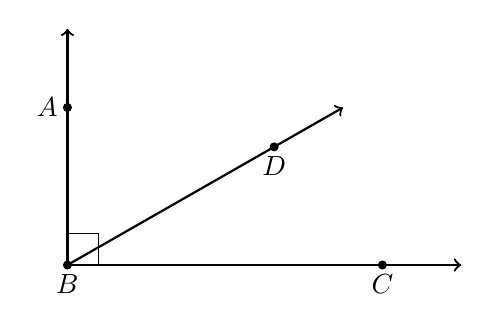
\begin{tikzpicture}[scale=1]
  \draw [<->, thick] (0,3)--(0,0)--(5,0);
  \draw [->, thick] (0,0)--(3.5, 2);
  \draw [-, thin] (0, 0.4)--(0.4, 0.4)--(0.4, 0);
  %\node at (3,.4){1};
  %\node at (6,-.6){2};
  \draw [fill] (0,0) circle [radius=0.05] node[below]{$B$};
  \draw [fill] (0,2) circle [radius=0.05] node[left]{$A$};
  \draw [fill] (4,0) circle [radius=0.05] node[below]{$C$};
  \draw [fill] (2.625, 1.5) circle [radius=0.05] node[below]{$D$};
\end{tikzpicture}
\end{flushleft}

\end{enumerate}
\end{document}
